\documentclass[12pt,a4paper]{article}

\usepackage[utf8]{inputenc}
\usepackage[T2A]{fontenc}
\usepackage[ukrainian]{babel}

\usepackage{geometry}
\geometry{left=2cm,right=2cm,top=2cm,bottom=2cm}

\usepackage{graphicx}
\usepackage{array,multirow}
\usepackage{booktabs}
\usepackage{caption}
\renewcommand{\thetable}{№\arabic{table}}
\captionsetup[table]{name=Таблиця}

\usepackage{amsmath}
\usepackage{pdflscape}
\usepackage{xcolor}
\usepackage{hyperref}

\begin{document}

    \begin{titlepage}

        % Картинка шапки (по центру, з відступом від верху)
        \begin{center}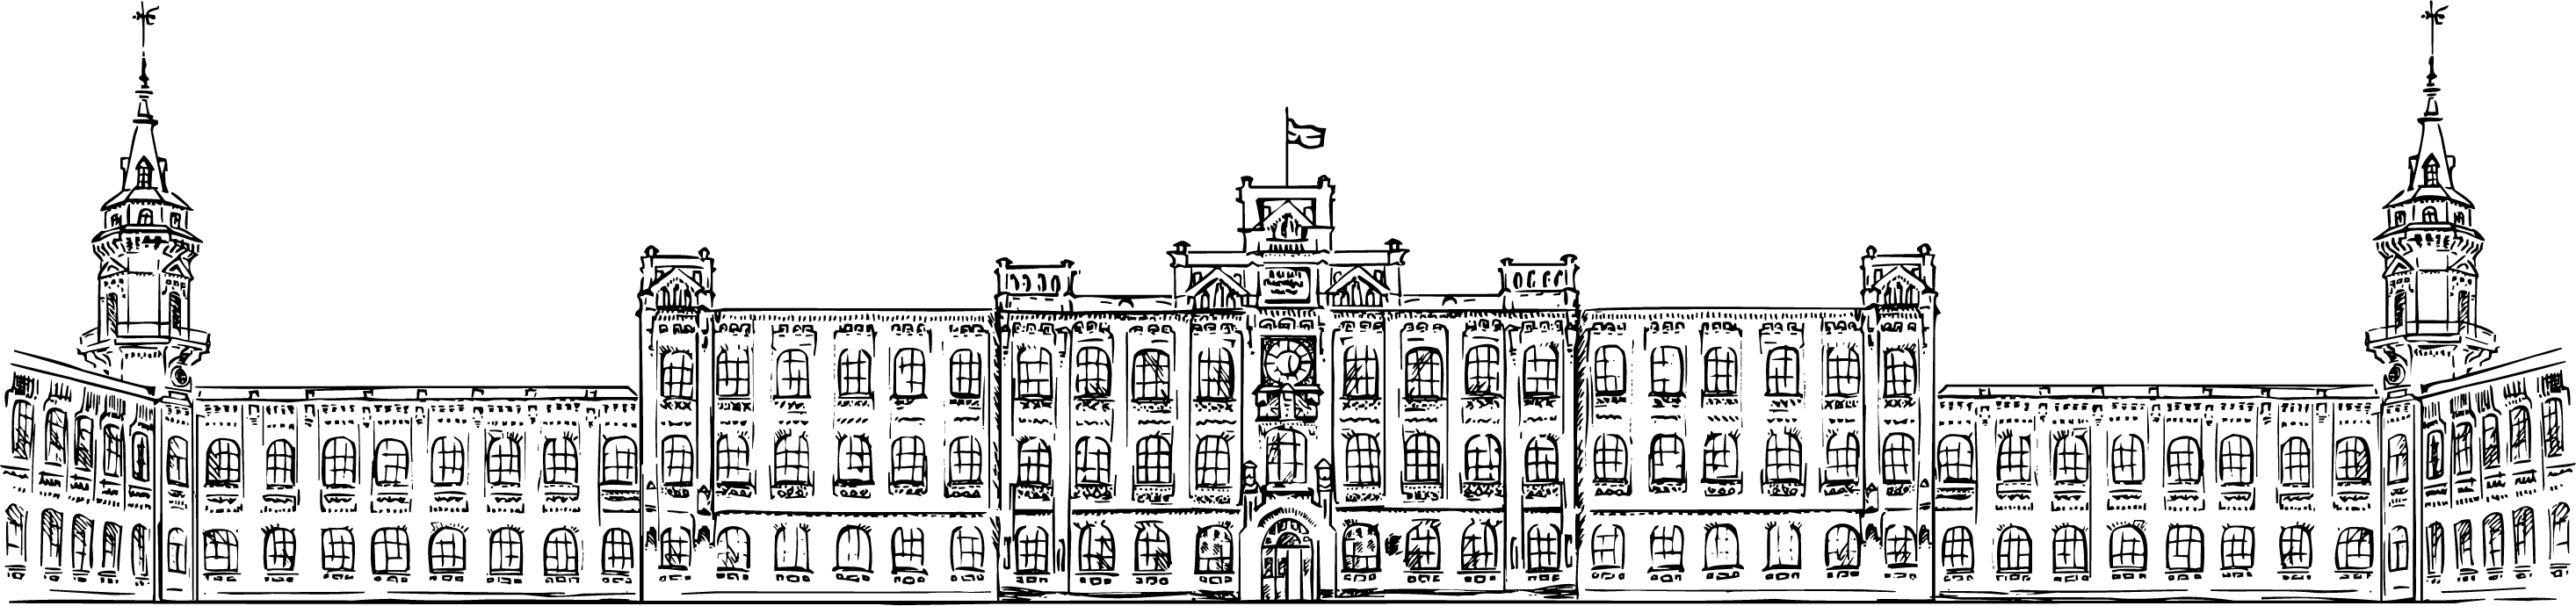
\includegraphics[width=0.7\textwidth]{../../../TITLES/letterhead.png}\end{center}

        \begin{center}
            \large Національний технічний університет України\\
            «Київський політехнічний інститут імені Ігоря Сікорського»\\[1em]
            Факультет інформатики та обчислювальної техніки\\
            Кафедра обчислювальної техніки
        \end{center}

        \vfill

        \begin{center}
            \textbf{\LARGE Психологія конфлікту}\\[2.5em]
            \textbf{\Large Тема 6. Типи конфліктів в організаціях}
        \end{center}

        \vfill

        \begin{flushright}
            Виконав: студент 2 курсу ФІОТ, гр. ІО-41\\
            \textit{Давидчук А.~М.}\\[1em]
            Перевірив: \textit{Папуша В.~В.}
        \end{flushright}

        \vfill

        \begin{center}Київ --- 2025\end{center}

    \end{titlepage}

    % ================= Основний текст =================

    \section*{Вступ}
    Жодна організація не існує без конфліктів. 
    Вони виникають у процесі розподілу ресурсів, прийняття рішень, взаємодії підрозділів і людей, 
    що виконують різні ролі та мають різні інтереси. 
    Водночас конфлікт в організації не є суто негативним явищем: 
    від того, як він протікає та як ним управляють, залежить, чи матиме він руйнівні чи конструктивні наслідки.

    Розуміння типів конфліктів в організаціях дає змогу:
    \begin{itemize}
        \item точніше діагностувати причини напруження;
        \item обирати адекватні стратегії втручання;
        \item попереджати ескалацію конфліктів;
        \item використовувати конфлікт як ресурс розвитку організації.
    \end{itemize}

    \section*{Поняття організаційного конфлікту}
    \textbf{Організаційний конфлікт}~--- це зіткнення інтересів, цілей, цінностей або способів діяльності учасників 
    організації (окремих працівників, груп, підрозділів, керівництва), пов’язане з виконанням ними своїх ролей та 
    функцій у структурі організації.

    Особливості організаційного конфлікту:
    \begin{itemize}
        \item він \textit{завжди пов’язаний з формальною структурою} (посади, повноваження, відповідальність);
        \item відбувається в межах \textit{регламентованих процедур} (накази, інструкції, посадові обов’язки);
        \item має \textit{економічні, управлінські й соціально-психологічні наслідки};
        \item впливає не лише на окремих працівників, а й на \textit{ефективність організації загалом}.
    \end{itemize}

    \section*{Типи конфліктів за рівнем організаційної структури}
    За рівнем, на якому виникає протиріччя, виділяють такі типи конфліктів:

    \subsection*{Внутрішньоособистісний конфлікт в організації}
    Виникає тоді, коли:
    \begin{itemize}
        \item вимоги до працівника суперечливі (\textit{рольовий конфлікт});
        \item реальні можливості не відповідають очікуванням керівництва або власним амбіціям;
        \item особисті цінності працівника не збігаються з нормами організації;
        \item людина перебуває в стані професійного вигорання чи хронічного стресу.
    \end{itemize}

    \subsection*{Міжособистісний конфлікт}
    Це конфлікт між окремими працівниками:
    \begin{itemize}
        \item між колегами одного рівня (горизонтальний конфлікт);
        \item між керівником та підлеглим (вертикальний конфлікт);
        \item між представниками різних підрозділів при особистому протистоянні.
    \end{itemize}

    Він часто стосується:
    \begin{itemize}
        \item стилю роботи й комунікації;
        \item розподілу навантаження й відповідальності;
        \item оцінки внеску кожного в спільний результат;
        \item особистісної несумісності.
    \end{itemize}

    \subsection*{Міжгруповий конфлікт}
    Включає протистояння:
    \begin{itemize}
        \item між підрозділами (відділами, департаментами, цехами);
        \item між формальними та неформальними групами;
        \item між адміністрацією й трудовим колективом.
    \end{itemize}

    Типові причини:
    \begin{itemize}
        \item конкурентна боротьба за ресурси, повноваження, вплив;
        \item різні критерії оцінки ефективності роботи;
        \item суперечливі цілі підрозділів (наприклад, \textit{відділ продажів} vs \textit{служба якості}).
    \end{itemize}

    \section*{Типи конфліктів за напрямом взаємодії}
    \subsection*{Вертикальні конфлікти}
    Виникають між представниками різних рівнів ієрархії:
    \begin{itemize}
        \item \textbf{«керівник~--- підлеглий»}: незгода з розподілом завдань, стилем керівництва, оцінюванням результатів;
        \item \textbf{«вища ланка керівництва~--- середня ланка»}: різні бачення стратегії, темпів змін, методів управління.
    \end{itemize}

    Особливості:
    \begin{itemize}
        \item нерівність формальної влади;
        \item ризик \textit{прихованих конфліктів} (зовнішня згода при внутрішньому спротиві);
        \item значний вплив стилю керівництва на характер і частоту конфліктів.
    \end{itemize}

    \subsection*{Горизонтальні конфлікти}
    Виникають між:
    \begin{itemize}
        \item колегами одного статусу;
        \item керівниками підрозділів, які мають однаковий рівень повноважень.
    \end{itemize}

    Типові підстави:
    \begin{itemize}
        \item розбіжності в підходах до виконання завдань;
        \item конкуренція за ресурси чи визнання;
        \item проблеми координації спільних проектів.
    \end{itemize}

    \subsection*{Змішані конфлікти}
    Поєднують горизонтальні та вертикальні елементи:
    \begin{itemize}
        \item залучають кілька рівнів ієрархії та підрозділів;
        \item можуть трансформуватися з міжособистісних у міжгрупові й навпаки;
        \item складніші для управління, оскільки мають розгалужену мережу учасників.
    \end{itemize}

    \section*{Типи конфліктів за змістом і предметом}
    \subsection*{Ресурсні конфлікти}
    Пов’язані з розподілом:
    \begin{itemize}
        \item фінансових ресурсів (бюджет підрозділу, премії, доплати);
        \item матеріальних ресурсів (обладнання, робочі місця, технології);
        \item людських ресурсів (штат, доступ до фахівців, розподіл персоналу по проектах);
        \item інформаційних ресурсів (доступ до даних, аналітики, контактів).
    \end{itemize}

    \subsection*{Рольові конфлікти}
    Виникають, коли:
    \begin{itemize}
        \item вимоги різних ролей суперечать одна одній (\textit{керівник і «свій» для колег});
        \item працівник не приймає нав’язану йому роль;
        \item організація постійно змінює функції співробітників без чітких правил і компенсацій.
    \end{itemize}

    \subsection*{Ціннісні та ідеологічні конфлікти}
    Пов’язані з:
    \begin{itemize}
        \item різними підходами до місії та цілей організації;
        \item відмінностями у професійній етиці, стандартах якості;
        \item конфліктом між \textit{формальними} цінностями організації та \textit{реальною практикою} (декларують одне, роблять інше).
    \end{itemize}

    \subsection*{Інформаційні конфлікти}
    Виникають унаслідок:
    \begin{itemize}
        \item дефіциту або надлишку інформації;
        \item суперечливих розпоряджень від різних керівників;
        \item невчасного інформування про зміни;
        \item викривлення інформації при її передачі по ієрархії.
    \end{itemize}

    \section*{Типи конфліктів за формою перебігу}
    \subsection*{Відкриті та приховані конфлікти}
    \textbf{Відкритий конфлікт}:
    \begin{itemize}
        \item явно виражені претензії, суперечки, зіткнення позицій;
        \item протистояння легко спостерігати зовні;
        \item є можливість \textit{прямо обговорювати} проблему.
    \end{itemize}

    \textbf{Прихований конфлікт}:
    \begin{itemize}
        \item зовнішньо зберігається видимість згоди;
        \item незадоволення проявляється через плітки, пасивний опір, саботаж;
        \item складніше для діагностики, але може мати \textit{більш руйнівні довгострокові наслідки}.
    \end{itemize}

    \subsection*{Конструктивні та деструктивні конфлікти}
    \textbf{Конструктивний конфлікт}:
    \begin{itemize}
        \item зосереджений на \textit{проблемі}, а не на особистості;
        \item веде до поліпшення процесів, уточнення цілей, підвищення ефективності;
        \item передбачає готовність сторін шукати взаємоприйнятні рішення.
    \end{itemize}

    \textbf{Деструктивний конфлікт}:
    \begin{itemize}
        \item спрямований на дискредитацію, приниження, усунення опонента;
        \item супроводжується ескалацією агресії, поляризацією груп;
        \item знижує ефективність роботи, руйнує довіру та командну взаємодію.
    \end{itemize}

    \section*{Типи конфліктів за тривалістю та інтенсивністю}
    \subsection*{Короткочасні та затяжні конфлікти}
    \textbf{Короткочасні конфлікти}:
    \begin{itemize}
        \item виникають у конкретній ситуації (наприклад, розподіл термінового завдання);
        \item можуть бути швидко вирішені через переговори або уточнення завдань;
        \item не завжди залишають глибокий слід у стосунках.
    \end{itemize}

    \textbf{Затяжні конфлікти}:
    \begin{itemize}
        \item тривають тривалий час, часто \textit{хвилеподібно} (загострення~--- затухання);
        \item пов’язані з глибинними ціннісними, статусними чи структурними протиріччями;
        \item формують \textit{стійкі коаліції} та ворожі підгрупи в колективі.
    \end{itemize}

    \subsection*{Низько- та високоінтенсивні конфлікти}
    \begin{itemize}
        \item \textbf{Низькоінтенсивні}~--- хронічне невдоволення, «прохолодні» стосунки, пасивний опір.
        \item \textbf{Високоінтенсивні}~--- відкриті конфронтації, сильні емоційні вибухи, різкі дії (звільнення, бойкот).
    \end{itemize}

    \section*{Значення класифікації конфліктів для управління організацією}
    Класифікація конфліктів в організаціях потрібна не лише для теоретичного опису, але й для практики управління:
    \begin{itemize}
        \item дозволяє \textit{швидко ідентифікувати} основний тип конфлікту;
        \item допомагає обрати \textit{відповідний інструментарій} втручання (переговори, медіація, зміна структури, корекція ролей);
        \item дає змогу \textit{відрізняти конфлікти, які варто приглушити}, від конфліктів, що можуть бути \textit{корисними для розвитку};
        \item використовується в \textit{діагностиці організаційної культури} й рівня конфліктності.
    \end{itemize}

    Ефективне управління організацією передбачає не уникнення будь-яких конфліктів, 
    а вміння \textit{переводити їх у конструктивну площину}, мінімізувати деструктивні наслідки та 
    використовувати як джерело інновацій, зворотного зв’язку і вдосконалення управлінських рішень.

    \section*{Висновки}
    В організаціях існує широкий спектр типів конфліктів: за рівнем структури, напрямом взаємодії, змістом, формою перебігу, 
    тривалістю та інтенсивністю. 
    Кожен тип має свої причини, динаміку та наслідки, що вимагає різних підходів до діагностики й розв’язання.

    Усвідомлення типів організаційних конфліктів дозволяє:
    \begin{itemize}
        \item зменшувати імовірність руйнівних ескалацій;
        \item підтримувати здоровий рівень робочих суперечок;
        \item будувати культуру відкритого обговорення проблем;
        \item підвищувати ефективність команди та організації загалом.
    \end{itemize}

    \section*{Список використаних джерел}
    \begin{enumerate}
        \item Бочарова С. П., Пасічник І. Д. \textit{Психологія конфлікту: навчальний посібник}. --- Київ: Академвидав, 2013.
        \item Гришина Н. В. \textit{Психология конфликта}. --- Санкт-Петербург: Питер, 2008.
        \item Немов Р. С. \textit{Психология: в 3 т. Т. 1. Общие основы психологии}. --- Москва: Владос, 2010.
        \item Роббінз С. П., Джадж Т. А. \textit{Організаційна поведінка}. --- К.: Основи, 2014.
        \item Томас К. \textit{Управление конфликтом}. --- Москва: Дело, 2000.
        \item Петровська Л. А. \textit{Психологія управління: навчальний посібник}. --- Київ: Центр учбової літератури, 2012.
    \end{enumerate}


\end{document}